\documentclass{beamer}
%% \documentclass[handout]{beamer}

\usetheme{default}

\usepackage[english]{babel}
\usepackage[latin1]{inputenc}

\usepackage{times}
\usepackage[T1]{fontenc}

%%
%%  some useful macro definitions & configuration settings
%%

\usepackage{latexsym}
\usepackage{graphicx}
\usepackage{url}
\usepackage{alltt}              % code examples with nicely formatted comments
\usepackage{xcolor}
\usepackage{pifont}
\usepackage{xspace}
\usepackage{array,booktabs}

\definecolor{quietred}{rgb}{.6,.2,.1}
\definecolor{quietblue}{rgb}{.1,.2,.7}
\definecolor{brightred}{rgb}{.9,0,.1}

%% > plot(x,y)      \REM{this produces a scatterplot}
\newcommand{\REM}[1]{\textsf{\small\color{quietred}\# #1}}

%% nice colour for R output: \begin{Rout} .. \end{Rout}
\newenvironment{Rout}{%
  \begin{footnotesize}\color{quietblue}\bfseries}{%
  \color{black}\mdseries\end{footnotesize}}

%% ... This is something \h{important}. ...
\newcommand<>{\h}[1]{\textbf#2{\color#2{quietred}#1}}
\newcommand<>{\hh}[1]{\textbf#2{\color#2{brightred}#1}}

%% cite \textcite{some text} in roman italic font
\newcommand{\textcite}[1]{\textrm{\textit{#1}}}

%% how can you live without the arrow (\so) and the hand (\hand) ?
\newcommand{\so}{\ding{234}\xspace}
\newcommand{\So}{\hh{\ding{229}}\xspace}
\newcommand{\hand}{\ding{43}\xspace}

%% \p{X=k};  \pC{X=k}{Y=l};  \bigp{X_i = k};   \pscale{\frac{Z}{S^2}};
%% probability P(X=k) and conditional probability P(X=k|Y=l), also with larger or scaled parentheses
%% \p[\theta]{X=k};  \pC[\text{interpolated}]{X=k}{Y=l};  ...
%% with optional subscripts (for model probability, null probability, etc.)
\newcommand{\p}[2][]{\mathop{\text{Pr}_{#1}}(#2)}
\newcommand{\pscale}[2][]{\mathop{\text{Pr}_{#1}}\!\left(#2\right)}
\newcommand{\bigp}[2][]{\mathop{\text{Pr}_{#1}}\bigl(#2\bigr)}
\newcommand{\pC}[3][]{\p[#1]{#2\,|\,#3}} 
\newcommand{\pCscale}[3][]{\pscale[#1]{#2\left|\,#3\right.\!}} 
\newcommand{\bigpC}[3][]{\bigp[#1]{#2\bigm|#3}} 

%% \Exp{X};  \Var{X};  \Exp[0]{X};  \Var[0]{X};  
%% \bigExp{X}; \bigVar{X}; \Expscale{X};  \Varscale{X};
%% expectation E[X] and variance V[X], expectation and variance under null hypothesis, 
%% and variants with largeer or scaled brackets
\newcommand{\Exp}[2][]{\text{E}_{#1}[#2]}
\newcommand{\Var}[2][]{\mathop{\text{Var}}_{#1}[#2]}
\newcommand{\bigExp}[2][]{\text{E}_{#1}\!\bigl[#2\bigr]}
\newcommand{\bigVar}[2][]{\mathop{\text{Var}}_{#1}\bigl[#2\bigr]}
\newcommand{\Expscale}[2][]{\text{E}_{#1}\left[#2\right]}
\newcommand{\Varscale}[2][]{\mathop{\text{Var}}_{#1}\left[#2\right]}


\title[SIGIL: Collocations 1]{Statistical Analysis of Corpus Data with R}
\subtitle{\emph{You shall know a word by the company it keeps!}\\
  Collocation extraction with statistical association measures\\
  --- Part 1 ---}

\author[Baroni \& Evert]{Designed by Marco Baroni\inst{1} and Stefan Evert\inst{2}}
\institute[]{
  \inst{1}Center for Mind/Brain Sciences (CIMeC)\\
  University of Trento
  \and
  \inst{2}Institute of Cognitive Science (IKW)\\
  University of Onsabr�ck
}
\date{}


\begin{document}

\frame{\titlepage}

 \begin{frame}
   \frametitle{Outline}
   \tableofcontents
 \end{frame}

%%%%%%%%%%%%%%%%%%%%%%%%%%%%%%%%%%%%%%%%%%%%%%%%%%%%%%%%%%%%%%%%%%%%%%%%

\section{Collocations \& Multiword Expressions (MWE)}

\newcommand{\tc}[1]{\textcite{\large #1}}
\begin{frame}
  \frametitle{What is a collocation?}

  \begin{itemize}
  \item Words tend to appear in typical, recurrent combinations:
    \begin{tabbing}
      $\quad$ \tc{day} \=and \tc{night} \\
      \> \tc{ring} \=and \tc{bell} \\
      \>\> \tc{milk} \=and \tc{cow} \\
      \>\>\> \tc{kick} \=and \tc{bucket} \\
      \>\>\>\> \tc{brush} and \tc{teeth}
    \end{tabbing}
  \item[] \pause
  \item[] \hand such pairs are called \h{collocations} (Firth 1957)
    \begin{itemize}
    \item the meaning of a word is in part determined by its characteristic
      collocations
    \item \emph{``You shall know a word by the company it keeps!''}
    \end{itemize}
  \end{itemize}
\end{frame}

\begin{frame}
  \frametitle{What is a collocation?}

  \begin{itemize}
  \item Native speakers have strong \& widely shared intuitions about such
    collocations
  \item[]
  \item Collocational knowledge is essential for non-native speakers in order
    to sound natural \so ``idiomatic English'' 
  \end{itemize}
\end{frame}

\begin{frame}
  \frametitle{An important distinction \ldots}
  \framesubtitle{\ldots\ which has been the cause of many misunderstandings.}

  \begin{itemize}
  \item \h{collocations} are an empirical linguistic phenomenon
    \begin{itemize}
    \item can be observed in corpora \& quantified
    \item provide a window to lexical meaning and word usage
    \item applications in language description (Firth 1957) and computational
      lexicography (Sinclair 1966, 1991)
    \end{itemize}
  \item[]\pause
  \item \h{multiword expressions} = lexicalised word combinations
    \begin{itemize}
    \item MWE need to be lexicalised (i.e., stored as units) because of
      certain idiosyncratic properties
    \item non-compositionallity, non-substitutability, non-modifiability
      (Manning \& Sch�tze 1999)
    \item not observable, defined by linguistic tests\\ (e.g.\ substitution
      test) and native speaker intuitions
    \end{itemize}
  \item[]\pause
  \item[\hand] the term ``collocations'' has been used for both concepts
  \end{itemize}
\end{frame}

\AtBeginSection[]{
  \begin{frame}<beamer:1| handout:0>
    \frametitle{Outline}
    \tableofcontents[current,currentsection]
  \end{frame}}

\AtBeginSubsection[]{
  \begin{frame}<beamer:1| handout:0>
    \frametitle{Outline}
    \tableofcontents[current,currentsubsection]
  \end{frame}}

%%%%%%%%%%%%%%%%%%%%%%%%%%%%%%%%%%%%%%%%%%%%%%%%%%%%%%%%%%%%%%%%%%%%%%%%

\subsection{What are collocations?}

\begin{frame}
  \frametitle{But what \emph{are} collocations?}

  \begin{itemize}
  \item Empirically, collocations are words that show an \h{attraction}
    towards each other (or a ``mutual expectancy'')
    \begin{itemize}
    \item in other words, a tendency to occur near each other
    \item collocations can also be understood as statistically salient
      patterns that can be exploited by language learners 
    \end{itemize}
  \item[]\pause
  \item Linguistically, collocations are an \h{epiphenomenon} \ldots\\\pause
    $\qquad$ \ldots\ some might also say a hotchpotch \ldots\\\pause
    \ldots\ of many different linguistic causes that lie behind the observed
    surface attraction.
  \end{itemize}
\end{frame}

\begin{frame}
  \frametitle{Collocates of \emph{bucket} (n.)}
  
  \begin{center}
    \begin{scriptsize}
      \begin{tabular}{>{\itshape}lr}
        \toprule
        \textup{noun} & $f$ \\
        \midrule
      water & 183 \\
      spade &  31 \\
    plastic &  36 \\
       slop &  14 \\
       size &  41 \\
        mop &  16 \\
     record &  38 \\
     bucket &  18 \\
        ice &  22 \\
       seat &  20 \\
       coal &  16 \\
    density &  11 \\
    brigade &  10 \\
  algorithm &   9 \\
     shovel &   7 \\
  container &  10 \\
       oats &   7 \\
       sand &  12 \\
      Rhino &   7 \\
  champagne &  10 \\
        \bottomrule
      \end{tabular}
      \hspace{5mm}
      \begin{tabular}{>{\itshape}lr}
        \toprule
        \textup{verb} & $f$ \\
        \midrule
      throw & 36 \\
       fill & 29 \\
  randomize &  9 \\
      empty & 14 \\
        tip & 10 \\
       kick & 12 \\
       hold & 31 \\
      carry & 26 \\
        put & 36 \\
      chuck &  7 \\
       weep &  7 \\
       pour &  9 \\
      douse &  4 \\
      fetch &  7 \\
      store &  7 \\
       drop &  9 \\
       pick & 11 \\
        use & 31 \\
       tire &  3 \\
      rinse &  3 \\
        \bottomrule
      \end{tabular}
      \hspace{5mm}
      \begin{tabular}{>{\itshape}lr}
        \toprule
        \textup{adjective} & $f$ \\
        \midrule
          large & 37 \\
  single-record &  5 \\
           cold & 13 \\
     galvanized &  4 \\
     ten-record &  3 \\
           full & 20 \\
          empty &  9 \\
       steaming &  4 \\
     full-track &  2 \\
   multi-record &  2 \\
          small & 21 \\
          leaky &  3 \\
     bottomless &  3 \\
     galvanised &  3 \\
           iced &  3 \\
          clean &  7 \\
         wooden &  6 \\
            old & 19 \\
       ice-cold &  2 \\
     anti-sweat &  1 \\
        \bottomrule
      \end{tabular}
    \end{scriptsize}
  \end{center}
\end{frame}

\begin{frame}
  \frametitle{Collocates of \emph{bucket} (n.)}

  \begin{itemize}
  \item opaque \h{idioms} (\emph{kick the bucket}, but often used literally)
  \item \h{proper names} (\emph{Rhino Bucket}, a hard rock band)
  \item noun \h{compounds}, lexicalised or productively formed\\
    (\emph{bucket shop}, \emph{bucket seat}, \emph{slop bucket}, \emph{champagne bucket})
  \item \h{lexical collocations} = semi-compositional combinations\\
    (\emph{weep buckets}, \emph{brush one's teeth}, \emph{give a speech})
  \item cultural \h{stereotypes} (\emph{bucket and spade})
  \item \h{semantic compatibility} (\emph{full, empty, leaky bucket};\\
    \emph{throw, carry, fill, empty, kick, tip, take, fetch a bucket})
  \item \h{semantic fields} (\emph{shovel, mop}; hypernym \emph{container})
  \item \h{facts} of life (\emph{wooden bucket}; \emph{bucket of water, sand, ice, \ldots})
  \item often sense-specific (\emph{bucket size}, \emph{randomize to a bucket})
    
  \end{itemize}
\end{frame}

\begin{frame}
  \frametitle{Operationalising collocations}

  \begin{itemize}
  \item Firth introduced collocations as an essential component of his
    methodology, but without any clear definition
    \begin{itemize}
    \item[] \textcite{Moreover, these and other technical words are given
        their `meaning' by the restricted language of the theory, and by
        applications of the theory in quoted works. \textup{(Firth 1957,
          169)}}
    \end{itemize}
  \item[]
  \item Empirical concept needs to be formalised and quantified
    \begin{itemize}
    \item intuition: collocates are ``attracted'' to each other, i.e.\
      they tend to occur near each other in text
    \item definition of ``nearness'' \so \h{cooccurrence}
    \item quantify the strength of attraction between collocates based on
      their recurrence \so cooccurrence \h{frequency}
    \end{itemize}
  \item[]
  \item[\hand] We will consider word pairs $(w_1,w_2)$ such as (\emph{brush},
    \emph{teeth})
  \end{itemize}
\end{frame}

%%%%%%%%%%%%%%%%%%%%%%%%%%%%%%%%%%%%%%%%%%%%%%%%%%%%%%%%%%%%%%%%%%%%%%%%

\subsection{Types of cooccurrence}

\begin{frame}
  \frametitle{Different types of cooccurrence}

  \begin{enumerate}
  \item \h{Surface cooccurrence}
    \begin{itemize}
    \item criterion: surface distance measured in word tokens
    \item words in a \emph{collocational span} around the node word,\\
      may be symmetric (L5, R5) or asymmetric (L2, R0)
    \item traditional approach in lexicography and corpus linguistics
    \end{itemize}
  \item[]\pause
  \item \h{Textual cooccurrence}
    \begin{itemize}
    \item words cooccur if they are in the same text segment\\
      (sentence, paragraph, document, Web page, \ldots)
    \item often used in Web-based research (\so Web as corpus)
    \end{itemize}
  \item[]\pause
  \item \h{Syntactic cooccurrence}
    \begin{itemize}
    \item words in a specific syntactic relation, e.g.
      \begin{itemize}
      \item adjective modifying noun
      \item subject / object noun of verb
      \item N \emph{of} N and similar patterns
      \end{itemize}
    \item suitable for extraction of MWE (Krenn \& Evert 2001)
    \end{itemize}
  \end{enumerate}
\end{frame}
  
\begin{frame}
  \frametitle{Types of cooccurrence: examples}
  \framesubtitle{Surface cooccurrence}

  \begin{itemize}
  \item \h{Surface cooccurrences} of $w_1$ = \emph{hat} with $w_2$ = \emph{roll}
    \begin{itemize}
    \item symmetric \underline{window} of four words (L4, R4)
    \item limited by sentence boundaries
    \end{itemize}
  \end{itemize}

  \begin{center}
    \colorbox{blue!20!white}{%
      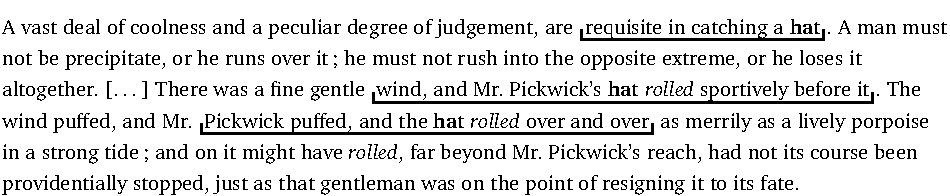
\includegraphics[width=\textwidth,height=3cm]{img/cooc_distance}}
  \end{center}

  \pause
  \begin{itemize}
  \item \h{coocurrence frequency} $f = 2$
  \item \h{marginal frequencies} $f_1 = f_2 = 3$
  \end{itemize}
\end{frame}

\begin{frame}
  \frametitle{Types of cooccurrence: examples}
  \framesubtitle{Textual cooccurrence}

  \begin{itemize}
  \item \h{Textual cooccurrences} of $w_1$ = \emph{hat} and $w_2$ = \emph{over}
    \begin{itemize}
    \item textual units = sentences
    \item multiple occurrences within a sentence ignored
    \end{itemize}
  \end{itemize}

  \begin{center}
    \colorbox{blue!20!white}{%
      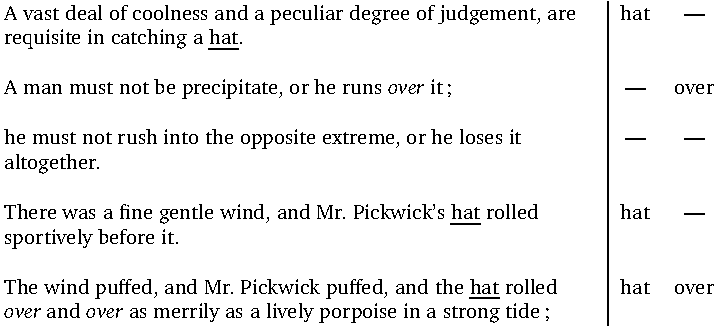
\includegraphics[scale=.7]{img/cooc_sentence}}
  \end{center}

  \pause
  \begin{itemize}
  \item coocurrence frequency $f = 1$
  \item marginal frequencies $f_1 = 3$,  $f_2 = 2$
  \end{itemize}
\end{frame}

\begin{frame}
  \frametitle{Types of cooccurrence: examples}
  \framesubtitle{Syntactic cooccurrence}

  \begin{itemize}
  \item \h{Syntactic cooccurrences} of adjectives and nouns
    \begin{itemize}
    \item every instance of the syntactic relation of interest is extracted as
      a \h{pair token}
    \end{itemize}
  \end{itemize}

  \begin{center}
    \colorbox{blue!20!white}{%
      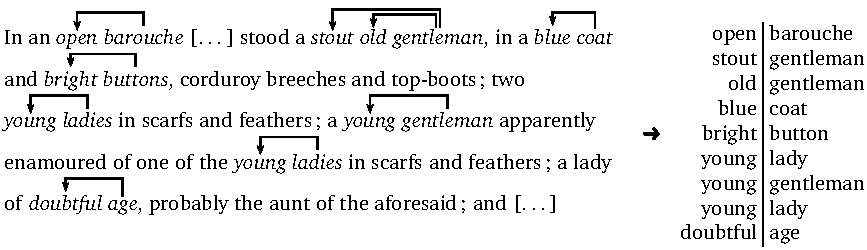
\includegraphics[scale=.7]{img/cooc_syntactic}}
  \end{center}

  \pause
  Cooccurrency frequency data for \emph{young gentleman}:
  \begin{itemize}
  \item coocurrence frequency $f = 1$
  \item marginal frequencies $f_1 = f_2 = 3$
  \end{itemize}
\end{frame}

%%%%%%%%%%%%%%%%%%%%%%%%%%%%%%%%%%%%%%%%%%%%%%%%%%%%%%%%%%%%%%%%%%%%%%%%

\section{Quantifying the attraction between words}

\begin{frame}
  \frametitle{Quantifying attraction}

  \begin{itemize}
  \item Quantitative measure for attraction between words based on their
    recurrence \so \h{cooccurrence frequency}%
    \pause
  \item But cooccurrence frequency is not sufficient
    \begin{itemize}
    \item bigram \emph{is to} occurs $f=$ 260 times in Brown corpus
    \item but both components are so frequent ($f_1\approx $ 10,000 and\\
      $f_2\approx $ 26,000) that one would also find the bigram 260 times if
      words in the text were arranged in completely random order
    \end{itemize}
    \pause%
    \hand take \h{expected frequency} into account as ``baseline''
  \item Statistical model required to bring in notion of ``chance
    cooccurrence'' and to adjust for sampling variation
  \item[]\pause 
    \begin{itemize}
    \item[\hand] NB: bigrams can be understood either as syntactic
      cooccurrences (adjacency relation) or as surface cooccurrences (L1, R0
      or L0, R1)
    \end{itemize}
  \end{itemize}
\end{frame}

\begin{frame}
  \frametitle{Attraction as statistical association}
  
  \begin{itemize}
  \item Tendency of events to cooccur = \h{statistical association}
    \begin{itemize}
    \item statistical measures of association are available for \h{contingency
        tables}, resulting from a \h{cross-classification} of a set of ``items''
      according to two (binary) factors
    \item cross-classifying factors represent the two events
    \end{itemize}
  \item[]\pause
  \item Application to word cooccurrence data
    \begin{itemize}
    \item most natural for \h{syntactic cooccurrences}
    \item ``items'' are pair tokens = instances of syntactic relation
    \item factor 1: Is first component of pair token an instance of word type
      $w_1$?
    \item factor 2: Is second component of pair token an instance of word type
      $w_2$?
    \end{itemize}
  \end{itemize}
\end{frame}

%%%%%%%%%%%%%%%%%%%%%%%%%%%%%%%%%%%%%%%%%%%%%%%%%%%%%%%%%%%%%%%%%%%%%%%%

\subsection{Contingency tables}

\begin{frame}
  \frametitle{Contingency table of observed frequencies}
  \framesubtitle{For \h{syntactic} cooccurrences}

  \centering

  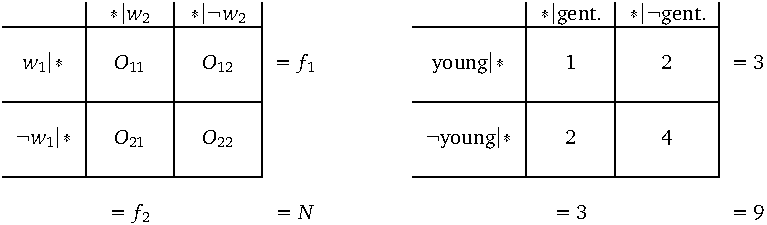
\includegraphics[width=\textwidth]{img/cont_table_syntactic}

  \vspace{1cm}
  \colorbox{blue!20!white}{%
    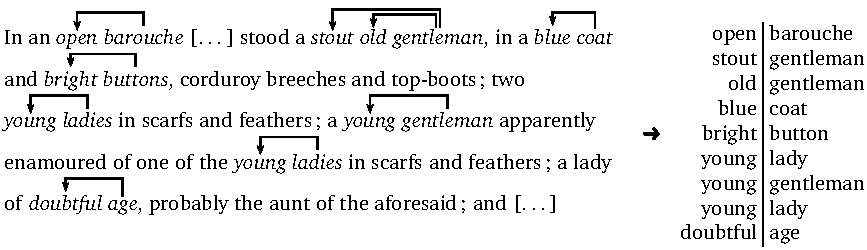
\includegraphics[scale=.6]{img/cooc_syntactic}}

\end{frame}

\begin{frame}
  \frametitle{Contingency table of observed frequencies}
  \framesubtitle{For \h{textual} cooccurrences (sentence windows)}

  \centering

  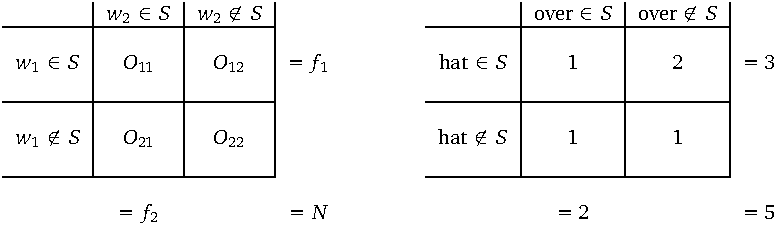
\includegraphics[width=\textwidth]{img/cont_table_sentence}

  \vspace{5mm}
  \colorbox{blue!20!white}{%
    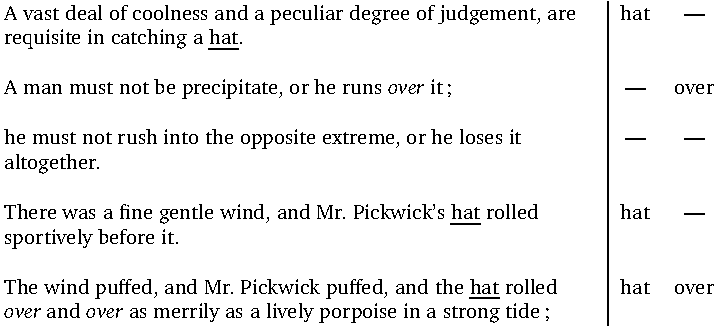
\includegraphics[scale=.6]{img/cooc_sentence}}

\end{frame}

\begin{frame}
  \frametitle{Contingency table of observed frequencies}
  \framesubtitle{For \h{surface} cooccurrences (L4, R4)}

  \centering

  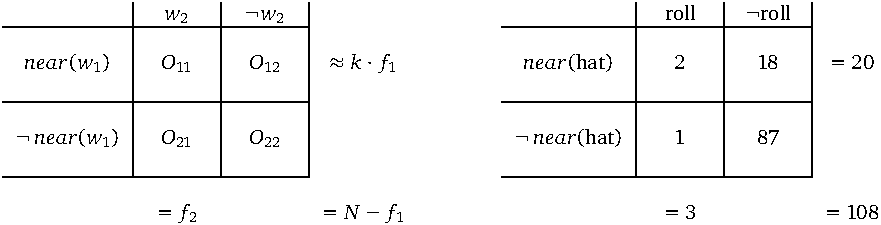
\includegraphics[width=\textwidth]{img/cont_table_distance}

  \vspace{5mm}
  \colorbox{blue!20!white}{%
    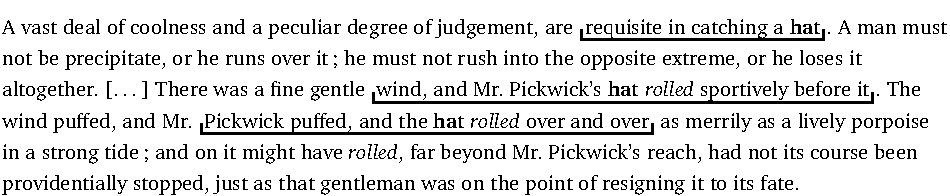
\includegraphics[scale=.6]{img/cooc_distance}}

  \vspace{5mm}
  \begin{footnotesize}
    \parbox{11cm}{%
      \h{More details:} Section 5.1 of Evert, S.\ (2008, in
      press). {\color{quietblue}Corpora and collocations.}  In A.~L{\"u}deling
      and M.~Kyt{\"o} (eds.), {\em Corpus Linguistics.  An International
        Handbook}, article~57. Mouton de Gruyter, Berlin.%
    }
  \end{footnotesize}

\end{frame}

\begin{frame}
  \frametitle{Measuring association in contingency tables}

  \begin{itemize}
  \item[A)] Measures of \h{significance}
    \begin{itemize}
    \item apply statistical hypothesis test with null hypothesis $H_0$:
      independence of rows and columns
    \item $H_0$ implies there is no association between $w_1$ and $w_2$
    \item \h{association score} = test statistic or p-value
    \item one-sided vs.\ two-sided tests
    \end{itemize}
    \hand amount of evidence for association between $w_1$ and $w_2$
  \item[]
  \item[B)] Measures of \h{effect-size}
    \begin{itemize}
    \item compare observed frequencies $O_{ij}$ to \h{expected frequencies}
      $E_{ij}$ under $H_0$ (\so later)
    \item or estimate conditional prob.\ $\pC{w_2}{w_1}$, $\pC{w_1}{w_2}$,
      etc.
    \item maximum-likelihood estimates or confidence intervals
    \end{itemize}
    \hand strength of the attraction between $w_1$ and $w_2$
  \end{itemize}
\end{frame}

%%%%%%%%%%%%%%%%%%%%%%%%%%%%%%%%%%%%%%%%%%%%%%%%%%%%%%%%%%%%%%%%%%%%%%%%

\subsection{Contingency tables and hypothesis tests in R}

\begin{frame}[fragile]
  \frametitle{Contingency tables in R}

  \begin{itemize}
  \item Contingency table is represented as a \h{matrix} in R,\\
    i.e.\ a rectangular array of numbers
    \begin{itemize}
    \item looks like numeric data frame, but different internally
    \end{itemize}
  \item E.g.\ for the following observed frequencies:\\
    $O_{11} = 9$, $O_{12} = 47$, $O_{21} = 82$, $O_{22} = 956$
  \end{itemize}
  \pause

  \begin{alltt}
> A <- matrix(c(10,47,82,956),
  nrow=2, ncol=2, byrow=TRUE)
> A

\REM{construct matrix from row (or column) vectors}
> A <- rbind(c(10,47), c(82,956))
  \end{alltt}
\end{frame}

\begin{frame}[fragile]
  \frametitle{Independence tests in R}

  \begin{alltt}
\REM{chi-squared test is the standard independence test}
> chisq.test(A)

\REM{use test statistic as association score, p-value for interpretation}

\REM{Is there significant evidence for a collocation?}

\REM{Fisher's exact test works better for small samples and skewed tables}
> fisher.test(A)
  \end{alltt}
\end{frame}

\begin{frame}
  \frametitle{Interpreting hypothesis tests as association scores}

  \begin{itemize}
  \item Establishing significance
    \begin{itemize}
    \item p-value = probability of observed (or more ``extreme'') contingency
      table if $H_0$ is true
    \item theory: $H_0$ can be rejected if p-value is below accepted
      \h{significance level} (commonly $.05$, $.01$ or $.001$)
    \item practice: nearly all word pairs are highly significant
    \end{itemize}
    \pause
  \item Test statistic = significance association score
    \begin{itemize}
    \item \h{convention} for association scores: high scores indicate strong
      attraction between words
    \item satisfied by \h{test statistic} $X^2$, but not by p-value
    \item Fisher's test: transform p-value, e.g.\ $-\log_{10} p$
    \end{itemize}
    \pause
  \item Odds ratio as measure of effect size
    \begin{itemize}
    \item Fisher's test also provides estimate for \h{odds ratio} $\theta$, an
      effect-size measure for association strength
    \item log odds ratio $\log \theta$ as effect-size association score\\
      (0 for independence, large values indicate strong attraction)
    \item conservative estimate = lower bound of confidence interval 
    \end{itemize}
  \end{itemize}
\end{frame}

\begin{frame}[fragile]
  \frametitle{Association scores from hypothesis tests}

  \begin{alltt}
\REM{chi-squared statistic \(X^2\) as association score}
> chisq.test(A)\$statistic

\REM{p-value of Fisher's test and corresponding association score}
> fisher.test(A)\$p.value
> -log10(fisher.test(A)\$p.value)

\REM{NB: chi-squared and Fisher scores are not on same scale}

\REM{log odds ratio and conservative estimate}
> log(fisher.test(A)\$estimate)
> log(fisher.test(A)\$conf.int[1])

> str(fisher.test(A))  \REM{or read help page carefully}
  \end{alltt}
\end{frame}

\begin{frame}[fragile]
  \frametitle{Association scores from hypothesis tests}

  \begin{alltt}
\REM{define two further (invented) contingency tables}
> B1 <- rbind(c(16,84), c(84,816))
> B2 <- rbind(c(1,99), c(99,801))

\REM{calculate chi-squared and Fisher scores for the two tables,}
\REM{as well as estimates for their log odds ratios}

\REM{Do the results look plausible to you? What is wrong?}
  \end{alltt}
\end{frame}

\begin{frame}[fragile]
  \frametitle{One-sided vs.\ two-sided association scores}

  \begin{itemize}
  \item Chi-squared and Fisher are \h{two-sided} tests
    \begin{itemize}
    \item calculate high association scores (= low p-values) both for strong
      positive association (\h{attraction}) and for strong negative
      association (\h{repulsion})
    \item we are usually interested in attraction only (unless we are looking
      for ``anti-collocations'')
    \end{itemize}
    \pause
  \item Fisher can be applied as \h{one-sided} test
    \begin{itemize}
    \item we are only interested in the \h{alternative} to $H_0$ that there is
      greater than chance cooccurrence, not in the alternative of less than
      chance cooccurrence
    \end{itemize}
  \end{itemize}
  
  \begin{alltt}
> fisher.test(B1, alternative="greater")    
\REM{high scores (significance and log odds ratio)}
> fisher.test(B2, alternative="greater")    
\REM{low scores (significance and log odds ratio)}
  \end{alltt}
\end{frame}

%%%%%%%%%%%%%%%%%%%%%%%%%%%%%%%%%%%%%%%%%%%%%%%%%%%%%%%%%%%%%%%%%%%%%%%%

\subsection{Practice session}

\begin{frame}
  \frametitle{Practice: bigrams in the Brown corpus}

  \begin{itemize}
  \item Data set of bigrams with $f\geq 5$ in the Brown corpus
    \begin{itemize}
    \item available on course homepage as \texttt{brown\_bigrams.tbl}
    \end{itemize}
  \item[]
  \item 24,167 rows (= bigrams) with variables:
    \begin{itemize}
    \item \h{id} = numeric ID of bigram
    \item \h{word1} = first word (e.g.\ \emph{long} for \emph{long time})
    \item \h{pos1} = part-of-speech code (e.g.\ \texttt{J} for adjective)
    \item \h{word2} = second word (e.g.\ \emph{time} for \emph{long time})
    \item \h{pos2} = part-of-speech code (e.g.\ \texttt{N} for noun)
    \item \h{O11} = observed cooccurrence frequency $O_{11}$
    \item \h{O12} = observed frequency $O_{12}$
    \item \h{O21} = observed frequency $O_{21}$
    \item \h{O22} = observed frequency $O_{22}$
    \end{itemize}
  \end{itemize}
\end{frame}

\begin{frame}[fragile]
  \frametitle{Practice: bigrams in the Brown corpus}

  \begin{alltt}
> Brown <- read.delim("brown_bigrams.tbl")

\REM{Now select a number of bigrams (e.g. low and high cooccurrence}
\REM{frequency, or specific part-of-speech combinations), construct}
\REM{the corresponding contingency tables in \texttt{matrix} form,}
\REM{and calculate the different association scores you know.}
\REM{Can you find a bigram with strong negative association?}

\REM{NB: You can use the same tests for corpus frequency comparisons.}
\REM{Assume that a certain expression occurs 50 times in the 100,000}
\REM{tokens of corpus A, and twice in the 1,000 tokens of corpus B.}
\REM{What is an appropriate contingency table for these data, and what}
\REM{results do you obtain from the chi-squared and Fisher test?}
  \end{alltt}
\end{frame}

%%%%%%%%%%%%%%%%%%%%%%%%%%%%%%%%%%%%%%%%%%%%%%%%%%%%%%%%%%%%%%%%%%%%%%%%

% \begin{frame}
%   \frametitle{}

% \end{frame}


\end{document}
